\section{双平方根方程的意义}
\label{sec:3.4}

双平方根方程具有石油勘探地震数据处理中大多数非统计方法方面的特点.这种在前一
节中导出的方程颇不易于理解,因为它是一种在四维空间$(z,s,g,t)$中的算子。我们将
通过各种具体应用来对它进行探讨,在各该应用中它均是一种较低维空间中的问题。在本节
中,速度横向变化将忽略不计(因为事情本来就够复杂的了,要考虑它就更棘手了)。讨论
就从下列二式开始:

\begin{subequations}
\begin{equation}
\frac{dU}{dz}=-\frac{i\omega}{v}[\sqrt{1-G^2}+\sqrt{1-S^2}]U
\label{eq:ex3.4.1a}
\end{equation}
\begin{equation}
\frac{dU}{dz}=-\frac{i\omega}{v}[\sqrt{1-(Y+H)^2}+\sqrt{1-(Y-H)^2}]U
\label{eq:ex3.4.1b}
\end{equation}
\label{eq:ex3.4.1}
\end{subequations}

\subsection{零炮检距偏移$(H=0)$}
\label{sec:3.4.1}

降低\ref{eq:ex3.4.1b}之维数的一种办法就是直接令$H=0$,于是两个平方根变得相同,从而
可将它们合并,得出熟悉的旁轴方程

\begin{equation}
\frac{dU}{dz}=i\omega\frac{2}{v}\sqrt{1-\frac{v^2k_y^2}{4\omega^2}}
\label{eq:ex3.4.2}
\end{equation}

在式\ref{eq:ex3.4.2}中出现岩石速度的两个地方,该岩石速度均应除以2,这是由于为使野外资料
与爆炸反射面模型相应,就需要使岩石速度减半。所以不论我们作过了什么,只要是令$H=0$,
我们就得到在第一章中使用过的方程了。令$H=0$就使观测排列延拓概念在作用上有等价于
爆炸反射面概念的效果了。

\subsection{零倾角叠加$(Y=0)$}
\label{sec:3.4.2}

处理炮检距$h$的时候,通常假设地层是水平成层的,从而观测结果将与中心点$y$无关。除
了或换句话说,除以外,采用这样一种地层模型时,所有遍及$y$之数据资料的
Fourier变换均将为零。当$Y=0$时,式\ref{eq:ex3.4.1}中的两个平方根又变得相等,因而所得方
程再一次成为旁轴方程

\begin{equation}
\frac{dU}{dz}=i\omega\frac{2}{v}\sqrt{1-\frac{v^2k_h^2}{4\omega^2}}
\label{eq:ex3.4.3}
\end{equation}

利用这个方程将双曲面从地表向下延拓时,可发现双曲面随着深度之增大而蜷缩,直至达到
出现最佳聚焦的正确深度,这种情形如图\ref{fig:ofs/dc2}所示。

各波均在零炮检距时出现最佳聚焦。出现聚焦代表向下延拓达到目的,这时,向下延拓
正好到达一个反射面。对于正位于反射面之上的自激自收点的情形,是在零值旅行时间上的
反射最强。采集$t=0$时在零炮检距上的值并放弃其余炮检距上的值,是消除干扰的一种途径
(实际上,这就是一种限制干扰影响的方法)。粗略地说,这同沿着原始资料上的双曲线轨
跡进行求和的常规处理过程就是一回事。很自然,向下延拓处理时采用的波速最接近于地层
速度时,求和可望达到最隹状态。以后就将利用炮检距空间来测定速度。


\subsection{常规处理---近似分离法}
\label{sec:3.4.3}

将式\ref{eq:ex3.4.1b}括号中的算子在形式上定义为双平方根算子(DSR算子)
\begin{equation}
\text{DSR}(Y,H)=\sqrt{1-(Y+H)^2}+\sqrt{1-(Y-H)^2}
\label{eq:ex3.4.4}
\end{equation}

\begin{figure}[H]
\centering
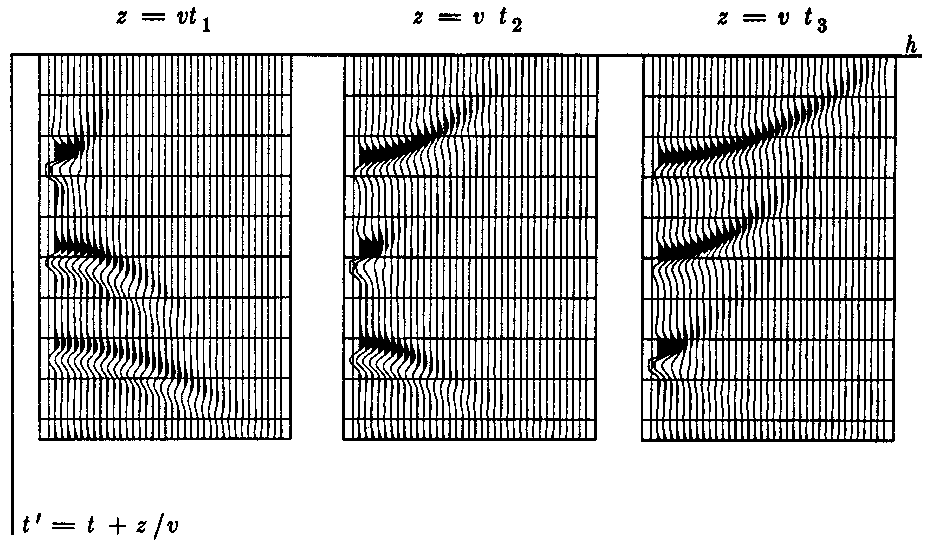
\includegraphics[width=0.65\textwidth]{ofs/dc2}
\caption[chervon]{采用三层的地层模型时,共中心点道集为三个双曲面。连续图形表示
向下延拓相继达到出现最佳聚焦时的深度}
\label{fig:ofs/dc2}
\end{figure}

在Fourie空间内,向下延拓是用相移因子$exp(i\omega \text{DSR}\frac{z}{v})$完成的。

采用这种算子有一个严重问题,无法将它分离成为一个炮检距算子与一个中心点算子之
和。不可分离的意思是,式\ref{eq:ex3.4.4}的Taylor级数展开中包含有像$Y^2H^2$这样的项,不能
把这样一些项表示成$Y$的一个函数加上$H$的一个函数,不可分离性是数据处理工作中的灾
难,它暗示着偏移与叠加必须同时完成而不能前后相继完成。要恢复纯粹的可分离性,其唯
一的途径就是回到$S$与$G$的空间中去(那可是远离常规处理的变化剧烈的抉择,我们将在以
后再转而讨论它)。

让我们回顾一下有关可分离性的一般性问题。为使算子$\sqrt{1-X^2-Y^2}$能近似分离,显
而易见的途径就是进行Taylor级数展开,然后略去所有交叉项,更精确的近似是
$\sqrt{1-X^2}+\sqrt{1-Y^2}-1$,它在$X=0$时准确地拟合于所有的$Y$,而在$Y=0$时则准确地拟合于所有的
$X$;把这个思想应用于双平方根算子,得

\begin{subequations}
\begin{equation}
\text{SEP}(Y,H)=2+[\text{DSR}(Y,0)-2]+[\text{DSR}(0,H)-2]
\label{eq:ex3.4.5a}
\end{equation}
\begin{equation}
\text{SEP}(Y,H)=2[1+(\sqrt{1-Y^2}-1)+(\sqrt{1-H^2}-1)]
\label{eq:ex3.4.5b}
\end{equation}


注意,在时,式\ref{eq:ex3.4.5}就等于双平方根算子;在$Y=0$时,该式也是等于双平方根
算子,仅当$H$与$Y$二者均非零时,SEP才不同于DSR。

式\ref{eq:ex3.4.5}分解成三个算子之和,能提供一种类似二维Fourier积分核$exp(ik_yy+ik_hh)$
所能提供的好处,该积分核具有的相位是由两部分之和所组成,这意味着Fouriei积分能够
对$y$或$h$按内嵌套循环进行处理。所以利用SEP进行向下延拓时,可以如式\ref{eq:ex3.4.1b}
所暗示的那样在$(k_h,k_y)$空间内完成,或者我们可以选定Fouriei变换,以适当的嵌套循环运算方
法变换至$(h,k_y)$、$(k_h,y)$或者$(y,h)$。

对式\ref{eq:ex3.4.5b}中的三项各取一个熟悉的名字是可带来方便的。第一项与时间深度转换
有关,第二项与偏移有关,第三项与正常时差有关;
\begin{equation}
\text{SEP}(Y,H)=\text{TD}+\text{MIG}(Y)+\text{NMO}(H)
\label{eq:ex3.4.5c}
\end{equation}
\label{eq:ex3.4.5}
\end{subequations}

可以把式\ref{eq:ex3.4.5}形式的近似解释为“标准处理”,标准处理中的第一步即是正常时
差校正。在式\ref{eq:ex3.4.5}中,NMO算子是将地表上的所有炮检距向下延拓为一定深度上的所
有炮检距。选择零炮检距只不过就是放弃所有其他炮检距;就同按炮检距进行叠加一样,选
择零炮检距可以减少所需考虑的数据量。

通常,被放弃的炮检距均不作偏移。相反,凡偏移之后改变叠加速度的精细处理都涉及
要对零炮检距附近的一些炮检距进行偏移。

既然SEP算子内的所有项均可相互交换,要是将它用于在叠加之前对所有炮检距迸行偏
移,那计算工作量似乎就太浪费了。梦样作所得结果将与叠后偏移完全一样。

\subsection{$H=0$的各种意义}
\label{sec:3.4.4}

时差算子$2H/v$有各种不同的形式:
\begin{equation*}
\frac{dt}{dh} ----- \text{射线轨迹情形下}
\end{equation*}
\begin{equation*}
\frac{k_h}{\omega} ----- \text{Fouder变换情形下}
\end{equation*}
\begin{equation*}
\partial_h^t=\int_{-\inf}^t dt\frac{\partial}{\partial h}-----\text{偏微分方程情形下}
\end{equation*}

互易性暗示着旅行时间〖为炮检距A的一个对称函数,从面在$h=0$时,$dt/dh$为零。在那
种意义下,把式\ref{eq:ex3.4.2}应用于零炮检距剖面看来是适宜的。更准确地说,射线轨迹表达
式严格说来只能在有一个平面波的时候才可应用。球形波阵面是由许多平面波之叠加
所形成。这时,关于$H$的Fouder变换解释要有稍许差别,而且更恰如其分。要挑选零频率
分量、即挑选地震记录道的平均值时,就令$\omega=0$;要挑选零空间频率分量,就是说,要挑选遍及
炮检距的求和,就令$k_h$=0。常规叠加可定义为沿某个双曲线轨迹遍及炮检距的积分或者求
和,直接令$k_h=0$就是挑选某个拉伸展平的双曲线轨迹,亦即速度为无限大时的双曲线。这
么一种积分或求和会接收到来自数据双曲面之顶部的主要影响,在该顶部,同相轴开始与进
行积分或求和所沿的水平直线相切。(由于若干历史原因,这样一种数据求和往往称为垂直
叠加)。在时差还没达到等于半波长之前,对积分的主要影响大多数是来自双曲线顶部邻近
的区域,称作Fresnel带的这种区域之宽度是影响该积分的主要因素。Fresnel带的概念已
在\ref{sec:1.2}节内介绍过了。图\ref{fig:ofs/denmark}所示是从一张野外剖面提取出的Fresnel带。

\begin{figure}[H]
\centering
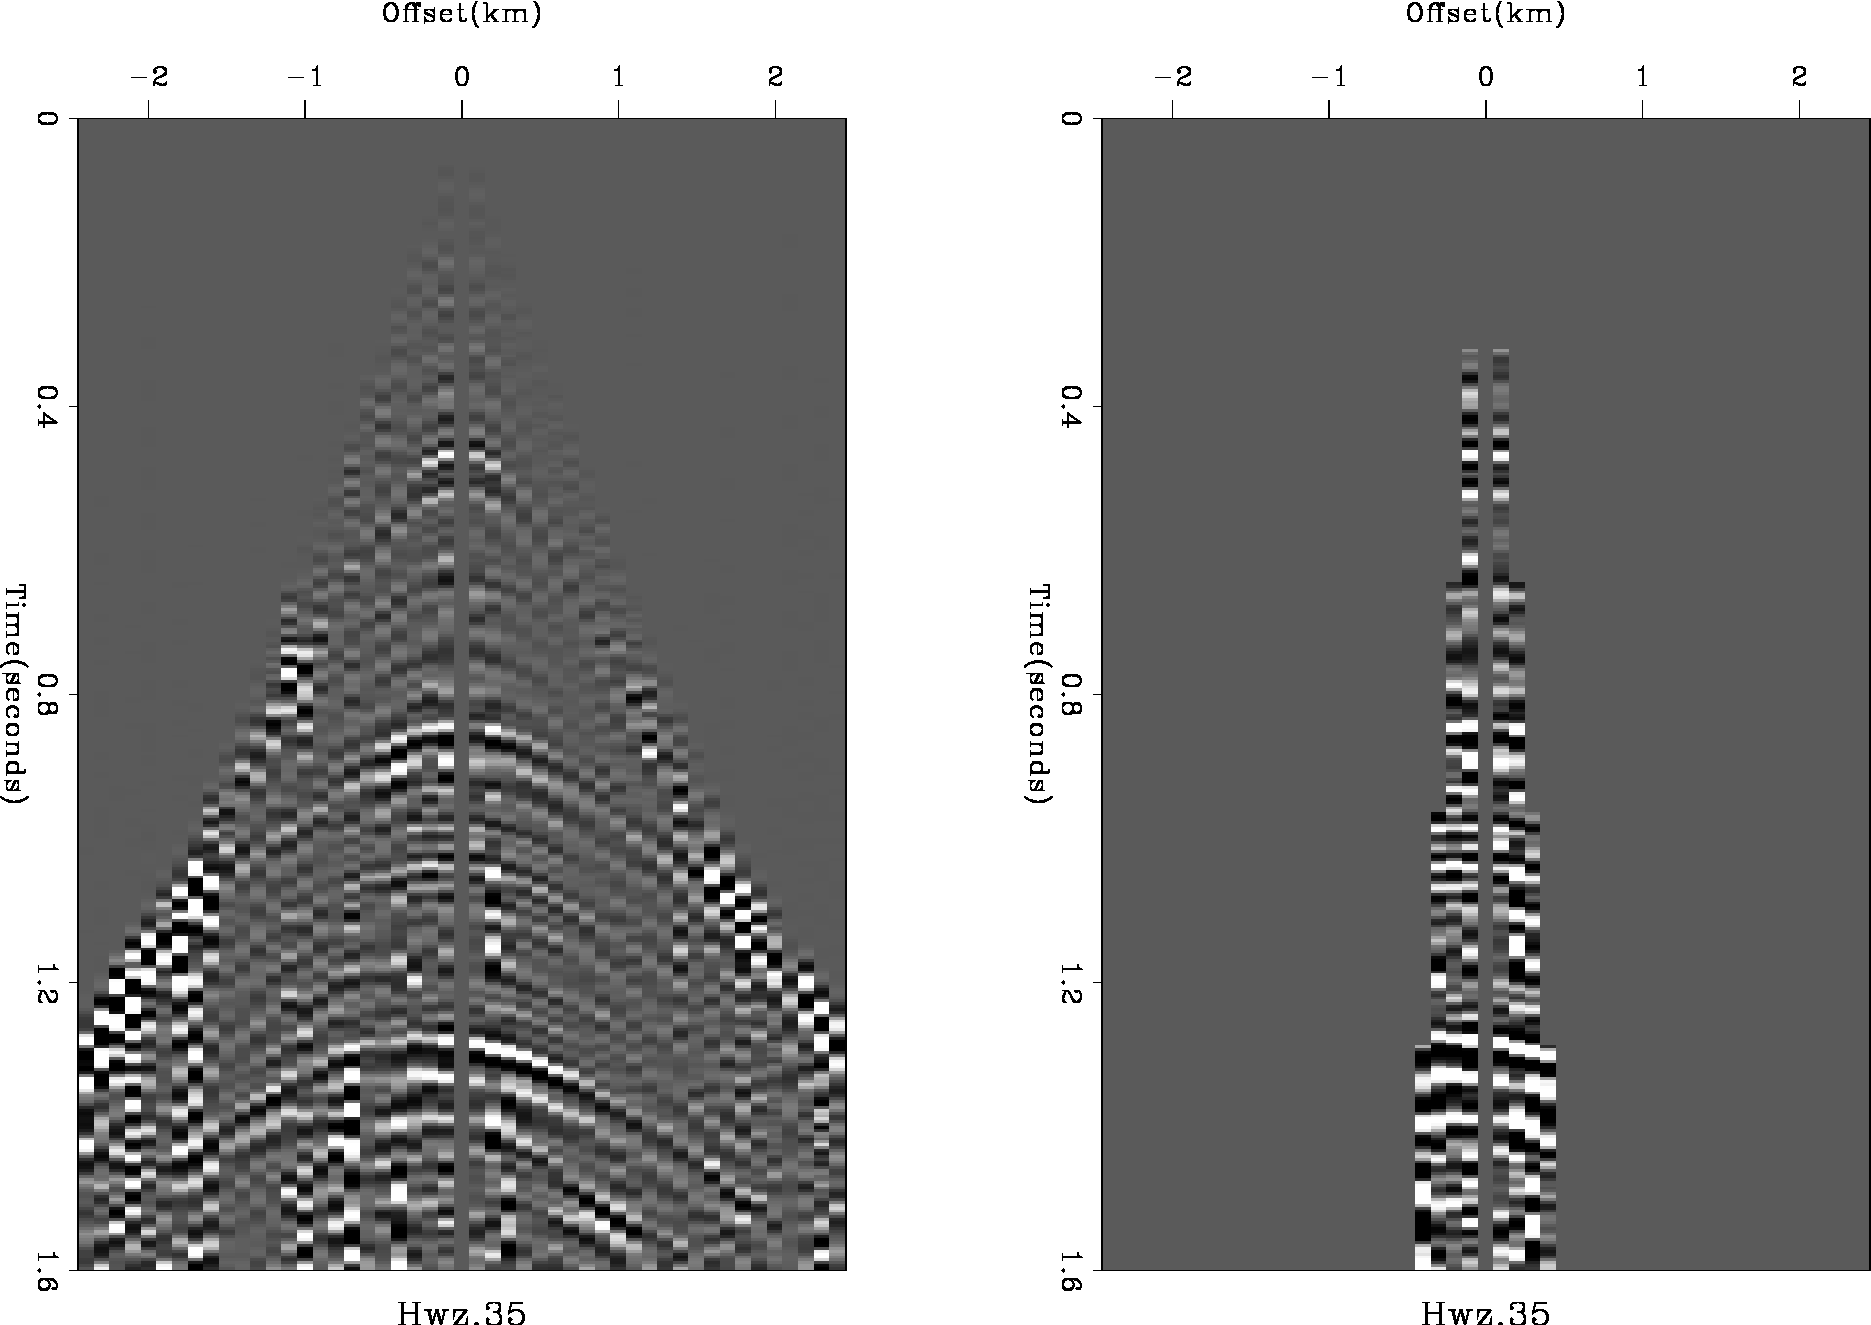
\includegraphics[width=0.65\textwidth]{ofs/denmark}
\caption[denmark]{丹麦某地区的陆地剖面(左图),由左图提取出并加以重新显示的
Fresnel带(右图)}
\label{fig:ofs/denmark}
\end{figure}

Fresnel带的定义必须涉及到某一种频率,就实用目的考虑,我们能够只考察几个零值交
点也就行了。仔细检查图\ref{fig:ofs/denmark}中1秒附近的记录,我们可看到有许多频率。在$t=1.0$至$t=1.1$
之间的间隔内,可看出大约有两种波长的低频和大约五种波长的高频。主要关心的是最高频
率,因为它们限定了地震分辨率的极限。自零时间至1秒时间之间所相应的深度大约为较高
频率所相应之半波长的100倍。作为一种概略的概念,可以说所观测到的这个值100适用于一
切旅行时间;那就是说,在任何旅行时间上,所观测到的具有空间可对比追踪性之最高频率
往往是具有一种大约为总旅行时间之1/100的半周期。我们可以说大地沉积地壳的品质因数Q
大约总是为100,所以我们典型考虑的角度大约为$cos8° = 0.99$。

从理论上来说,零炮检距剖面与垂直叠加之间的主要差别在于振幅不同并有某种微小的
相移。在实际处理情形下,它们看上去并不像是以显著不同的方式迸行偏移的。对于按照有
限速度而非无限大速度进行叠加的资料,如果我们能够找到一种实现向下延拓的方程那就好
了。

当速度是水平坐标的恒定函数时,令$H=0$这件事从偏微分方程的观点看来和从Fourier
变换的观点看来,是完全相同的;但是在其他情形时,偏微分方程观点就是更普遍一点的观
点。为了具体化而又不产生混乱,可将方程\ref{eq:ex3.4.1b}近似表示成适用于15°倾角、具有时
间滞后的空间域形式

\begin{equation}
[\frac{\partial}{\partial z}+\frac{v}{-i\omega 8}(\frac{\partial^2}{\partial y^2}+\frac{\partial^2}{\partial h^2})]U'=0
\label{eq:ex3.4.6}
\end{equation}

将这个方程遍及炮检距进行积分。积分算子与微分算子可互换。记住,微商的积分等于积
分上限计算所得函数与积分下限计算所得函数之差,因而得
\begin{subequations}
\begin{equation}
(\frac{\partial}{\partial z}+\frac{v}{-i\omega 8}\frac{\partial^2}{\partial y^2})
(\int Udh)+\frac{v}{-i\omega g}\frac{\partial U}{\partial h}\mid_{h=-\inf}^{h=+\inf}=0
\label{eq:ex3.4.7a}
\end{equation}

在无限大炮检距$h=±\inf$之处,波应消失,从而其对水平炮检距之导数也应等于零,
由此可知,式\ref{eq:ex3.4.7a}中的最后一顼应等于零。所以,令$H=0$就是意味着下列关系成立
\begin{equation}
(\text{旁轴算子})(\text{垂直叠加})=0
\label{eq:ex3.4.7b}
\end{equation}
\end{subequations}
建立式\ref{eq:ex3.4.7b}时有一个问题,即它已经两次假设速度与炮检距无关。第一次是当从式
\ref{eq:ex3.4.6}中忽略掉薄透镜项时第二次是在把炮检距积分的算子乘以速度作互换时。如
果速度同水平义轴有关,则它肯定就要与中心点和炮检距二者都有关。总之,如果速度在
Fresnel带的范围内是缓慢变化的,则取$H=0$就是为垂直叠加资料的向下延拓提供了一种有效的偏移方程。

\subsection{Clayton余弦校正}
\label{sec:3.4.5}

有这样一种可能性存在:使地层倾角之正
弦与$Y$有关,使炮检距所张角度之正弦与$H$有
关,当这种关系大致成立的时候,得进行一种
重耍的校正。试考虑图\ref{fig:ofs/clay}所示的倾斜地层。

反射面倾角为$\alpha$,炮检距可逋过炮检距角
度$\beta$来表达。我们将不加证明地引用Clayton所曾指出的下列关系:
\begin{subequations}
\begin{equation}
Y=sin\alpha cos\beta
\label{eq:ex3.4.8a}
\end{equation}
\begin{equation}
Y=sin\alpha cos\beta
\label{eq:ex3.4.8b}
\end{equation}
\label{eq:ex3.4.8}
\end{subequations}

在正角或负角很小的情形下,可将余弦略
去,这时使地层倾角$\alpha$之正弦与$Y$联系起来、使炮检距角度$\beta$之正弦与$H$联系起来,那是正确
的。在中等大小的角度时,则需要进行余弦校正,如式\ref{eq:ex3.4.8}所示。当角度超出45°时。
灵敏度反向,因而事情就颠倒混乱了。读者应当提防简单地把$Y$同倾角联系起来、把$H$同速
度联系起来的这种不正规讨论。倾角和炮检距可以混合发生影响,\ref{sec:3.2}节中的“Larner条
瘕”就是一个例子。实际上,在陡倾角时,利用$H$来确定塋变的这种普通处理办法应当以某
科方式使之改变为利用$Y$来进行。

\begin{figure}[H]
\centering
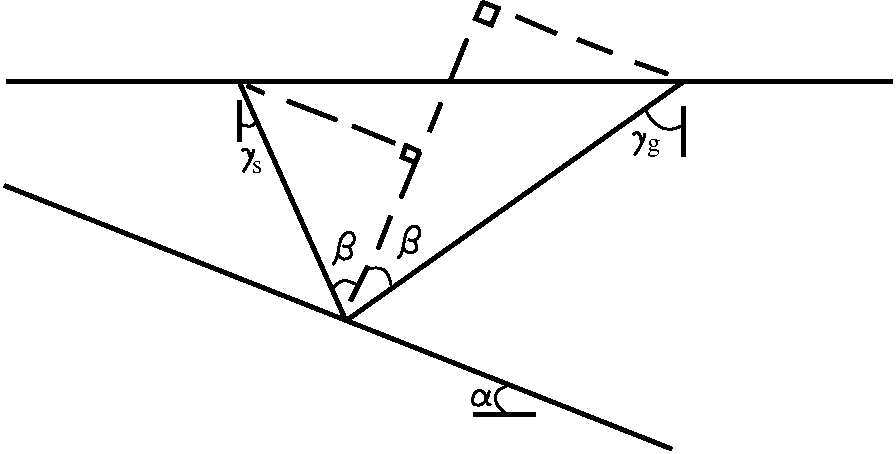
\includegraphics[width=0.65\textwidth]{ofs/clay}
\caption[clay]{倾斜地层几何形态。注意,角度$2\beta$的平分线并不通过$g$与$s$之间的中心点(Clayton)}
\label{fig:ofs/clay}
\end{figure}

接下去我们就来证明式\ref{eq:ex3.4.8}的关系。震源出射角为$\gamma_s$,入射至接收点的角度为
$\gamma_g$。首先,使$\gamma_s$与$\gamma_g$,同$\alpha$与$\beta$发生关系,将图\ref{fig:ofs/clay}中所作出的较小之三角形的所有角相加起来,得

\begin{equation*}
(-\frac{\pi}{2}-\gamma_s-\alpha)+\beta+\frac{\pi}{2}=\pi
\end{equation*}
\begin{subequations}
\begin{equation}
\gamma_s=\beta-\alpha
\label{eq:ex3.4.9a}
\end{equation}
把较大一个三角形的所有角相加起来,得
\begin{equation}
\gamma_g=\beta+\alpha
\label{eq:ex3.4.9b}
\end{equation}
\label{eq:ex3.4.9}
\end{subequations}

要把一定深度时的角度$\alpha$和$\beta$同地表上的时差$dt/ds$和$dt/dg$联系起来,需要告心符号之正负,
注意旅行时间之随检波点向右移而增大、随炮点向右移而减小。根据\ref{sec:3.3}节中的方程\ref{eq:ex3.3.16}
和\ref{eq:ex3.3.18}以及视倾角$Y$和$H$的定义,应有
\begin{equation*}
Y-H=S=\frac{vk_s}{\omega}=v\frac{dt}{ds}=-sin\gamma_s=sin(\alpha-\beta)
\end{equation*}
\begin{equation*}
Y+H=G=\frac{vk_g}{\omega}=v\frac{dt}{dg}=+sin\gamma_g=sin(\alpha+\beta)
\end{equation*}
将上述一对方程相加和相减,然后利用三角学的合角公式,得出Clayton的余弦校正公式\ref{eq:ex3.4.8}
\begin{equation*}
Y=\frac{1}{2}sin(\alpha+\beta)+\frac{1}{2}sin(\alpha-\beta)=sin\alpha cos\beta
\end{equation*}
\begin{equation*}
H=\frac{1}{2}sin(\alpha+\beta)-\frac{1}{2}sin(\alpha-\beta)=sin\beta cos\alpha
\end{equation*}

\subsection{Snell波叠加与共中心点道集倾斜叠加}
\label{sec:3.4.6}

令出射角S等于零,也就是把双平方根方程简化成单平方根方程了。$S=0$的意思是$k_s =
0$、或是其等价的意义:将数据遍及所有炮点$s$进行求和(无需时移而求和)。这样一种求和
相当于是模拟下行平面波,该求和过程幕后所隐含的成像原理是要找出在下行波到达时间上
出现的上行波(\ref{sec:5.7})。从历史渊源说,这就是我的CDP叠加剖面有限差分波动方程偏
移所隐含的思想。如以后在\ref{sec:5.2}节和\ref{sec:5.3}节中所阐述的,也可令$S$等于
一个常数以模拟下行Snell波。

Snell波是非垂直入射下行平面波的一种推广,炮点不是同时起爆,而是与$dt/ds$=$S/v$
成反比地相继起爆。通过$(t,s)$平面沿着斜率为心$dt/ds$的直线对野外资料进行求和,即可
模拟这种情形。令$S$为某种常数,例如也就是把双平方根方程简化为旁轴波动
方程,上述假想观测的下行Snell波向下延拓所需要的正是这个方程。Snell波能够用各种不
同的值$p=dt/ds$来构制,可各自偏移并成像,然后把所成的像遍及所有$p$进行叠加。早在双
平方根方程提出之前就已经产生这些思想了,可是至今它们尚未得到流行,其原因何在?

与模拟Snell波有关的一个问题就是:波场通常是沿检波器电缆方向按粗网格间隔加以
采样的,电缆长度本身几乎从未超出波传播的距离。在共检波点道集中,双曲线的顶部并不
需要位于零炮检距上,对数据进行内插与外推的精巧方法因此而失效。对于倾斜地层,最尽
到达的波至往往要偏离排列的墙点,所以数据处理因缺失数据而受到很大影响。

共中心点道集倾斜叠加、即$H=pv$,就是为了避免这些困雄而有了用武之地(关于倾
斜叠加的完整解释,见\ref{sec:5.2}节)。在其中心点上,双曲线以零斜率通过零炮检距,因而数据
更适合于沿一条倾斜直线迸行积分时所需采用的内插与外推运算。令$H=pv$,得
\begin{equation}
k_z=-\frac{\omega}{v}[\sqrt{1-(Y+pv)^2}+\sqrt{1-(Y-pv)^2}]
\label{eq:ex3.4.10}
\end{equation}
这个关系已经不能由双平方根方程简化为旁轴波动方程,值是它却使问题归结为一种易于
采用现成可用技术的形式了,诸如采用Stolt方法或者相移法等,这种处理办法的细节可参
阅Richard Ottolini的博士论文(1982)。

\subsection{为何不在(S,G)空间内向下延拓?}
\label{sec:3.4.7}

如果速度已知,因而仅有的任务只是偏移的话,这时不能在(S,G)空间内完成向下
延拓的基本理由就不存在了。可是,速度实际上总不是完全已知的。偏移对速度误差影响的
灵敏度随角度而迅速增大,因而得假设(S,G)空间内有相当的角度精度。此外,记录电
缆的有限长度范围以及出现空间假频的可能,均使(S,G)空间内的偏移遇到了与Snell叠加
所遭遇的相同问题。我看没什么重要理由可以使人相信(S,G)空间的偏移就是要比共中
心点道集倾斜叠加好一点,而且假频和截断误差的影晌看来似乎还使它更为糟糕。少为人知
但更实际的处理广角偏移问题的办法将在本章以后几节中讨论。

另一方面,速度有横向变化(如可已知的话),则可能需要在(s,
g)空间内来实现偏移。

采用炮点检波点空间还有另一个原因,这就是炮点彼此相距很远。这时数据无论在中心
点空间或炮检距空间内,都耍受到假频影响(见\ref{sec:5.7}节)。
